\documentclass{article}

\usepackage[utf8]{inputenc}
\usepackage[T1]{fontenc}
\usepackage[francais]{babel}

\usepackage{graphicx}			% Images

\usepackage{wrapfig}

\author{Thibaud \textsc{Colas}}
\date{\today}
\title{\LaTeX}


\begin{document}

\maketitle
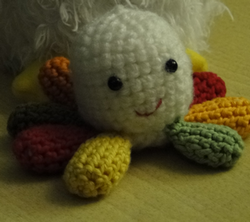
\includegraphics{poulpy.png}
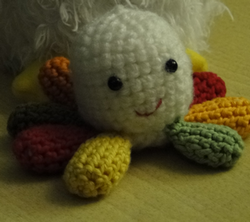
\includegraphics[width=200px]{poulpy.png}
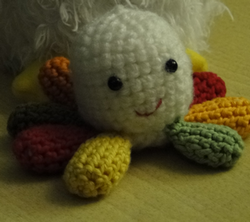
\includegraphics[height=200px]{poulpy.png}
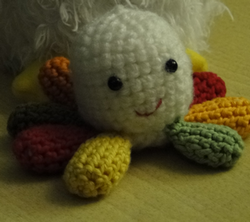
\includegraphics[height=200px, width=600px]{poulpy.png}  %Ici poulpy est un peu plate
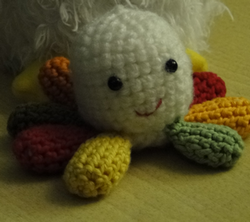
\includegraphics[scale=1.5]{poulpy.png}  %Ici poulpy est plutôt grande
	

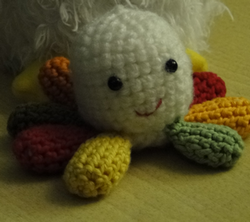
\includegraphics[angle=45]{poulpy.png} %poulpy en biais

%\includegraphics*[120,20][400,251]{poulpy_et_mr_poule.eps}



\begin{wrapfigure}[8]{r}{4cm}
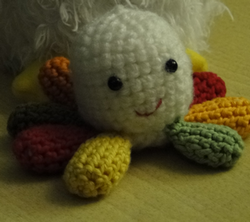
\includegraphics[width=4cm]{poulpy.png}
\end{wrapfigure}
Lorem ipsum dolor sit amet, consectetur adipiscing elit. Ut sit amet lectus a odio condimentum porttitor ac cursus orci. Aenean at sapien turpis. Fusce sollicitudin dictum tellus placerat porta. Curabitur lacinia consequat quam. Cras dapibus, sem vitae posuere facilisis, turpis sem facilisis arcu, quis ornare urna risus quis justo. Nunc sagittis blandit lectus sit amet ultrices.
Curabitur lacinia consequat quam. Cras dapibus, sem vitae posuere facilisis, turpis sem facilisis arcu, quis ornare urna risus quis justo. Nunc sagittis blandit lectus sit amet ultrices. 


\begin{figure}
\begin{center}
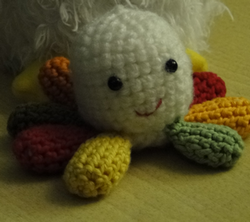
\includegraphics{poulpy.png} 
\end{center}

\end{figure}

\begin{figure}
\begin{center}
 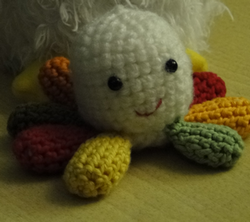
\includegraphics{poulpy.png} 
\end{center}
 \caption{Poulpy est multicolore}
 \label{Poulpy est multicolore}

\end{figure}

\clearpage % Nouvelle page et force les flottants à s'afficher avant la suite.
\cleardoublepage


\end{document}
